
\documentclass[12pt, a4paper]{article}
\usepackage{fullpage}
\usepackage{graphicx}
\usepackage{wrapfig}
\usepackage{amsmath}
\usepackage{float}
\usepackage{listings}
\usepackage{lmodern}  % for bold teletype font
\usepackage{xcolor}   % for \textcolor

\definecolor{codegreen}{rgb}{0,0.6,0}
\definecolor{codegray}{rgb}{0.5,0.5,0.5}
\definecolor{codepurple}{rgb}{0.58,0,0.82}
\definecolor{backcolour}{rgb}{0.95,0.95,0.92}

\title{\textbf{EE2703 : Applied Programming Lab \\ Assignment 10}} % Title

\author{Potta Muni Asheesh \\ EE19B048} % Author name

\date{\today} % Date for the report

\begin{document}	
\lstset{
  language=Python,
  backgroundcolor=\color{backcolour},   
  commentstyle=\color{codegreen},
  keywordstyle=\color{magenta},
  numberstyle=\tiny\color{codegray},
  stringstyle=\color{codepurple},
  basicstyle=\ttfamily,
  breakatwhitespace=false,         
  breaklines=true,                 
  captionpos=b,                    
  keepspaces=true,                 
  %numbers=left,                    
  %numbersep=5pt,                  
  showspaces=false,                
  showstringspaces=false,
  showtabs=false,                  
  tabsize=2,
  columns=fullflexible,
  frame=single,
  postbreak=\mbox{\textcolor{red}{$\hookrightarrow$}\space},
}	
		
\maketitle % Insert the title, author and date

\section{Introduction}

In this assignment, the computation of spectra of non-periodic signals is explored.

\section{Spectrum of $sin(\sqrt{2}t)$}

Consider the signal $y(t) = sin(\sqrt{2}t)$ sampled over the interval $[-\pi, \pi)$ at sampling rate $F_s = 64/2\pi$ and $y(-t_{max})$ is set to 0, to maintain the purely imaginary nature of spectra of sine waves.

\begin{lstlisting}
def ex1():
    t=np.linspace(-np.pi,np.pi,65);t=t[:-1]
    dt=t[1]-t[0];fmax=1/dt
    y=np.sin(np.sqrt(2)*t)
    y[0]=0 # the sample corresponding to -tmax should be set zero
    y=fftshift(y) # make y start with y(t=0)
    Y=fftshift(fft(y))/64.0
    w=np.linspace(-np.pi*fmax,np.pi*fmax,65);w=w[:-1]
\end{lstlisting}

The spectrum obtained is

\begin{figure}[H]
\centering
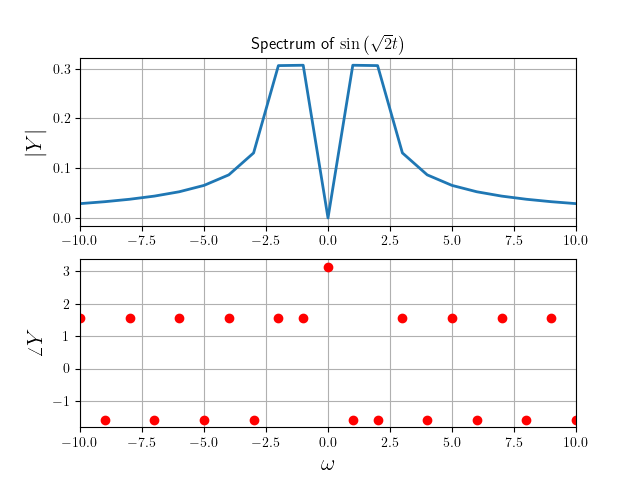
\includegraphics[width=0.8\textwidth]{ex1.png}
\end{figure}

Two spikes were expected. There are two spikes, but they are broad and the magnitude decays after the spikes. The phase corresponding to the spikes is correctly obtained.

To understand what went wrong. Consider the signal over the interval $[-3\pi, 3\pi)$.

\begin{figure}[H]
\centering
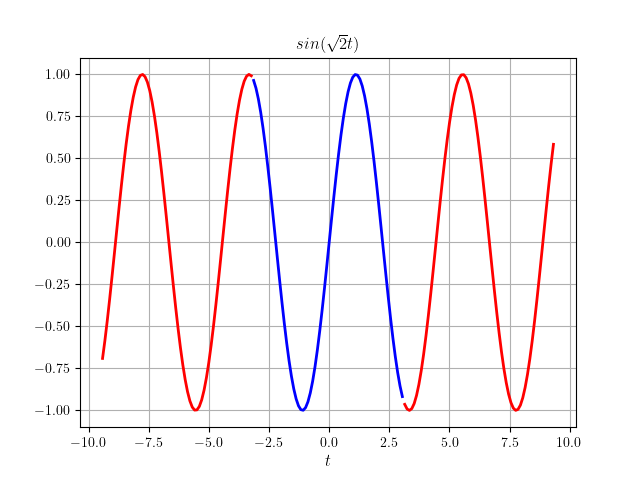
\includegraphics[width=0.8\textwidth]{ex2.png}
\end{figure}

It can be observed that the signal is periodic, but the part between $-\pi$ and $\pi$ is not the repeating part. Consider the signal obtained by wrapping $sin(\sqrt{2}t)$ every $2\pi$, which is the signal for which the spectrum has been obtained above.

\begin{figure}[H]
\centering
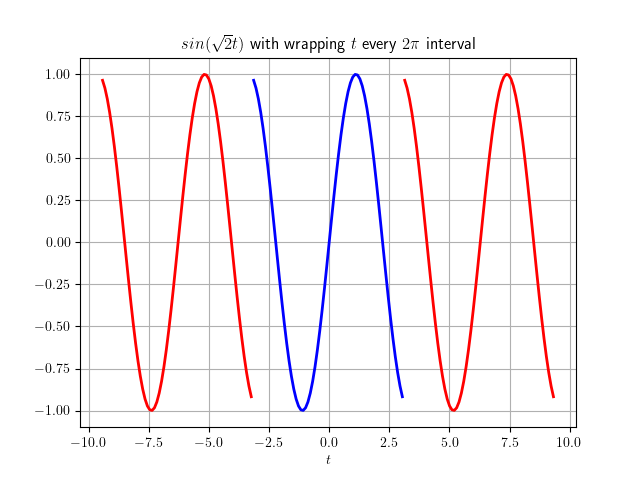
\includegraphics[width=0.8\textwidth]{ex3.png}
\end{figure}

It can be observed that there are jump discontinuities at every period and due to these jumps, the magnitude spectrum sees a gradual decay after the spikes. This is called \textbf{Gibbs phenonmenon}.

\subsection{Gibbs phenomenon}

It is observed in the spectra of signal which have discontinuities. Consider the periodic ramp signal for example.

\begin{equation*}
y(t) = t, -\pi < t < \pi
\end{equation*}

\begin{figure}[H]
\centering
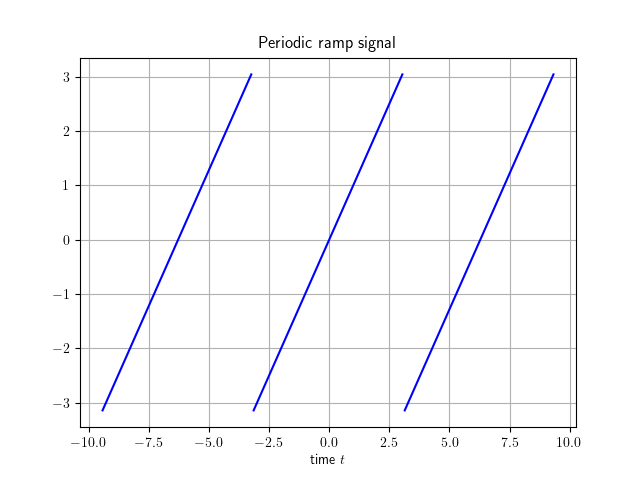
\includegraphics[width=0.8\textwidth]{ex4_1.png}
\end{figure}

The fourier series of this signal is 

\begin{equation*}
y(t) = 2\left( \frac{sin(t)}{1} - \frac{sin(2t)}{2} + \frac{sin(3t)}{3} - ... \right)
\end{equation*}

So, the spectrum decays as $1/\omega$ and the same is obtained, i.e; a -20dB/decade decay.

\begin{figure}[H]
\centering
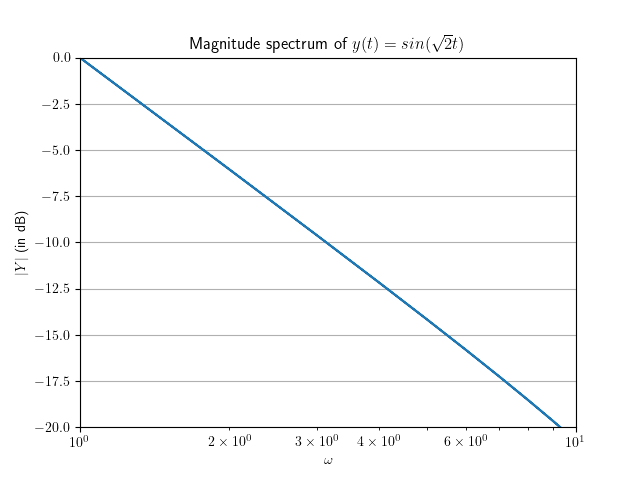
\includegraphics[width=0.8\textwidth]{ex4_2.png}
\end{figure}

\begin{lstlisting}
def ex4():
    t = np.linspace(-np.pi, np.pi, 65); t = t[:-1]
    t2 = np.linspace(-3*np.pi, -np.pi, 65); t2 = t2[:-1]
    t3 = np.linspace(np.pi, 3*np.pi, 65); t3 = t3[:-1]
    dt = t[1]-t[0]
    fmax = 1/dt
    y = t
    y[0] = 0
    y = fftshift(y)
    y_spec = fftshift(fft(y))/64.0
    w = np.linspace(-np.pi*fmax, np.pi*fmax, 65); w = w[:-1]
\end{lstlisting}

So, in order to reduce the affect of this phenomenon, \textbf{windowing} is used.

\subsection{Windowing}

In order to suppress the jump, the signal is multiplied by another sequence called \textit{window}.

\begin{equation*}
g(n) = f(n)w(n)
\end{equation*}

Multiplication in time domain results in convolution in frequency domain. The spectrum of the signal obtained is different from the actual spectrum required.

One of the window sequence is the \textit{hamming window}. It is given as

\begin{lstlisting}
def hamming_window(N):
    n = np.arange(N)
    return fftshift(0.54 + 0.46*np.cos(2*np.pi*n/(N-1)))
\end{lstlisting}

The plot of $sin(\sqrt{2}t) \times w(t)$ wrapped every $2\pi$ time is shown below.

\begin{figure}[H]
\centering
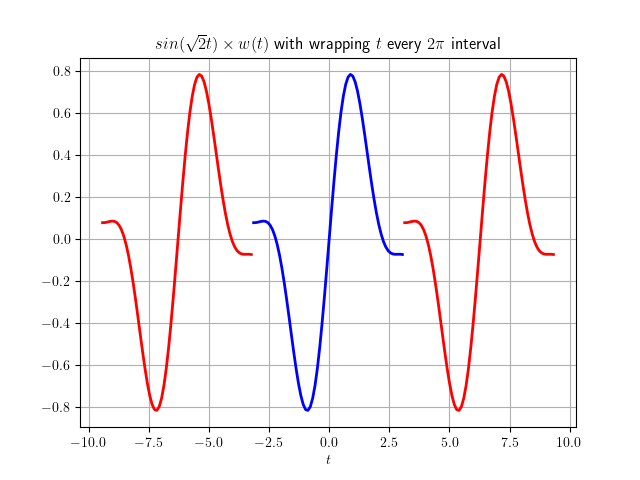
\includegraphics[width=0.8\textwidth]{ex5.png}
\end{figure}

The spectrum of this sequence is given as

\begin{figure}[H]
\centering
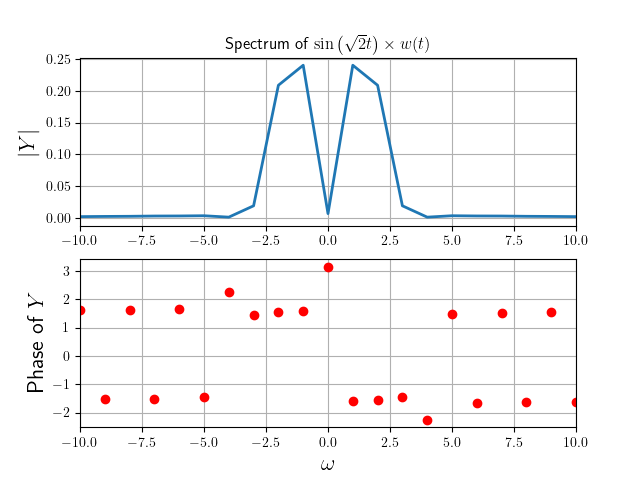
\includegraphics[width=0.8\textwidth]{ex6.png}
\end{figure}

The gradual decay in magnitude is not observed, but peak is still broad.

Now, four times the number of points are considered to get better resolution.

\begin{figure}[H]
\centering
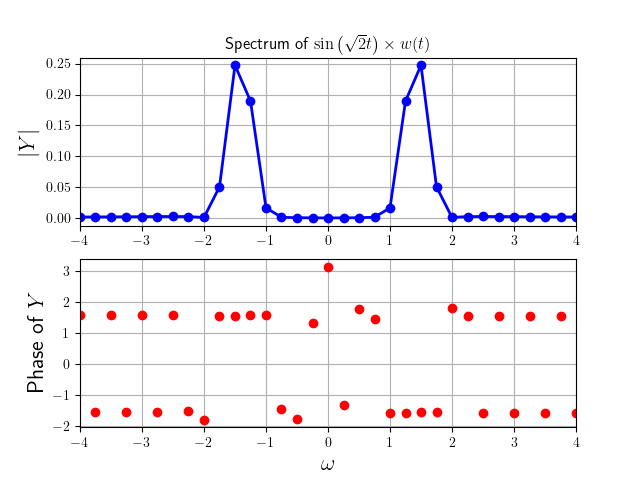
\includegraphics[width=0.8\textwidth]{ex7_1.png}
\end{figure}

The resolution has certainly improved, but it should be noted that the peak is still broad and this is because of the windowing, not only because $\sqrt{2}$ is between 1 and 2. To confirm this, the spectrum of $sin(1.5t) \times w(t)$ is also broad.

\begin{figure}[H]
\centering
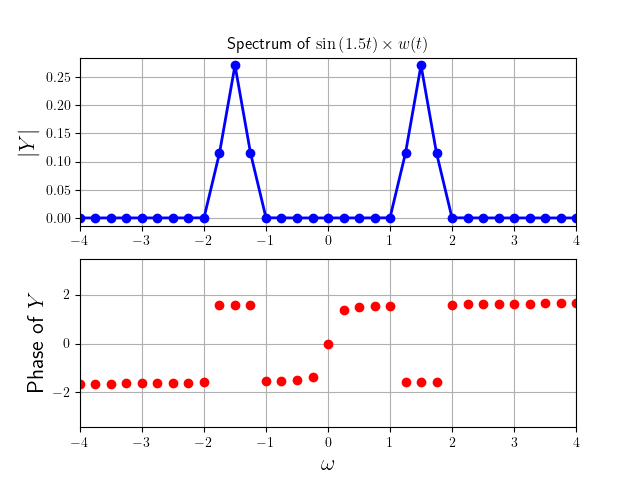
\includegraphics[width=0.8\textwidth]{ex7_2.png}
\end{figure}

\section{Spectrum of $cos^3(\omega_0 t)$}

Consider the signal $cos^3(\omega_0 t)$ with $\omega_0 = 0.86$.

The spectrum of this signal without a hamming window is given as 

\begin{figure}[H]
\centering
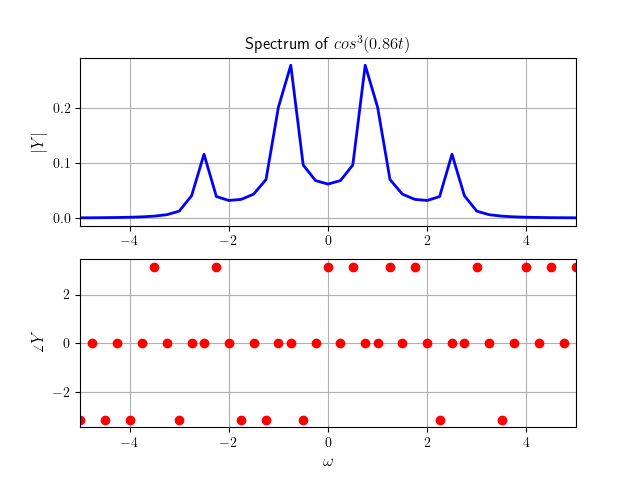
\includegraphics[width=0.8\textwidth]{q2_1.png}
\end{figure}

Now, the spectrum of this signal with a hamming window is given as

\begin{figure}[H]
\centering
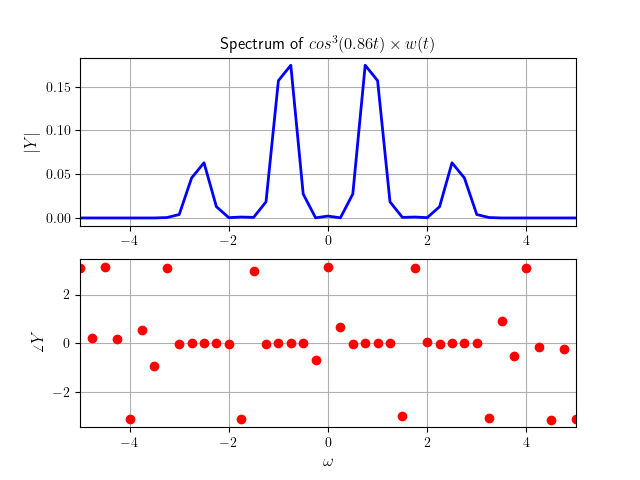
\includegraphics[width=0.8\textwidth]{q2_2.png}
\end{figure}

It can be observed that the windowing has certainly improved the magnitude spectrum.

\section{Estimating $\omega_0$ and $\delta$ in $cos(\omega_0 t + \delta)$}

A signal $cos(\omega_0 t + \delta)$ with arbitrary $\delta$ and $0.5 < \omega_0 < 1.5$ of length 128 samples can be generated as

\begin{lstlisting}
def arbit_cos(noise=False):
    t = np.linspace(-np.pi, np.pi, 129); t = t[:-1]
    w0 = np.random.rand() + 0.5
    delta = np.random.rand()*2*np.pi
    # if delta-np.pi > 0:
    #     delta = 2*np.pi - delta
    if noise:
        return t, np.cos(w0*t + delta) + 0.1*np.random.randn(128), w0, delta
    return t, np.cos(w0*t + delta), w0, delta
\end{lstlisting}

The frequency corresponding to peak in the spectrum is estimate for $\omega_0$ and the phase corresponding to this frequency is the estimate for $\delta$.

\begin{lstlisting}
def q3():
    t, y, w0, delta = arbit_cos()
    dt = t[1] - t[0]
    y[0] = 0
    y = fftshift(y)
    y_spec = fftshift(fft(y))/128
    y_spec_mag = np.abs(y_spec)
    y_spec_ang = np.angle(y_spec)
    w = np.linspace(-np.pi/dt, np.pi/dt, 129); w = w[:-1]
    ii = np.where(y_spec_mag == np.max(y_spec_mag))
    est_w0, est_delta = w[ii][-1], y_spec_ang[ii][-1]
    print('actual w0 and estimated w0 are {}, {}'.format(w0, est_w0))
    print('actual delta and estimated delta are {}, {}'.format(delta, est_delta))
\end{lstlisting}

Some of the estimates found are shown below.

\begin{itemize}
\item Actual $\omega_0$ and estimated $\omega_0$ are 0.5139319849138658, 1.0. Actual $\delta$ and estimated $\delta$ are 5.2899223447339185, -1.248008220373927.
\item Actual $\omega_0$ and estimated $\omega_0$ are 1.0692624800488058, 1.0. Actual $\delta$ and estimated $\delta$ are 0.397228803727542, 0.37904375462634254.
\item Actual $\omega_0$ and estimated $\omega_0$ are 0.5724358016556333, 0.0.
Actual $\delta$ and estimated $\delta$ are 0.14840584305304158, 0.0
\end{itemize}

It can be observed that frequency estimate is not very accurate due to resolution of the spectrum, but the phase is better estimated.

Silimar method is used to estimate, when white gaussian noise is added to signal.

\begin{lstlisting}
def q4():
    t, y, w0, delta = arbit_cos(noise=True)
    dt = t[1] - t[0]
    y[0] = 0
    y = fftshift(y)
    y_spec = fftshift(fft(y))/128
    y_spec_mag = np.abs(y_spec)
    y_spec_ang = np.angle(y_spec)
    w = np.linspace(-np.pi/dt, np.pi/dt, 129); w = w[:-1]
    ii = np.where(y_spec_mag == np.max(y_spec_mag))
    est_w0, est_delta = np.abs(w[ii][-1]), y_spec_ang[ii][-1]
    if est_delta < 0:
        est_delta += 2*np.pi
    print('Actual $\omega_0$ and estimated $\omega_0$ are {}, {}'.format(w0, est_w0))
    print('Actual $\delta$ and estimated $\delta$ are {}, {}'.format(delta, est_delta))
\end{lstlisting}

Some of the estimates found are shown below.

\begin{itemize}
\item Actual $\omega_0$ and estimated $\omega_0$ are 1.10588175592206, 1.0.
Actual $\delta$ and estimated $\delta$ are 1.0784816041319503, 1.0277791200791555
\item Actual $\omega_0$ and estimated $\omega_0$ are 1.3940422549339684, 1.0.
Actual $\delta$ and estimated $\delta$ are 4.880580976127553, 1.3076057592874013
\item Actual $\omega_0$ and estimated $\omega_0$ are 1.152667662320201, 1.0.
Actual $\delta$ and estimated $\delta$ are 2.446344906917355, 2.500639994772733
\end{itemize}

It can be seen that the estimate are not as accurate as they were when no noise is added. Hencen the noise makes estimation harder.

\section{Spectrum of Chirp signal}

Consider the signal

\begin{equation*}
y(t) = cos \left( 16 \left( 1.5 + \frac{t}{2\pi} \right) t \right)
\end{equation*}

This signal is called \textit{Chirped signal}. 

\begin{figure}[H]
\centering
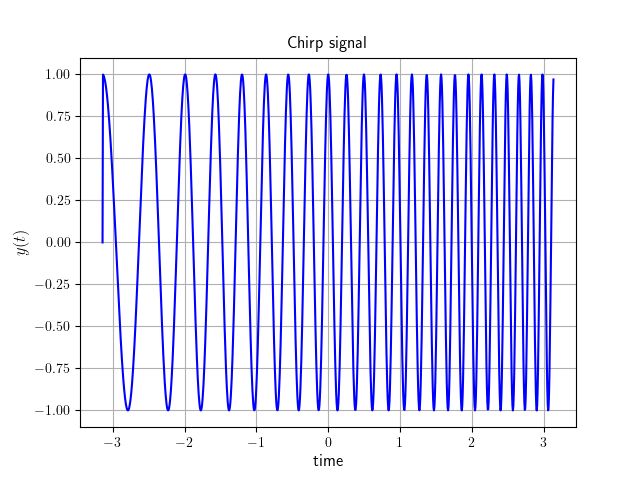
\includegraphics[width=0.8\textwidth]{q4_1.png}
\end{figure}

It can observed from the plot and equation that angular frequency gradually increases from 16 rads/s to 32 rads/s as time goes from $-\pi$ to $\pi$

The spectrum of this signal is obtained as,

\begin{lstlisting}
def q5():
    t = np.linspace(-np.pi, np.pi, 1025); t = t[:-1]
    dt = t[1] - t[0]
    y = np.cos(16*(1.5 + t/(2*np.pi))*t)
    y[0] = 0
    # y = fftshift(y)
    y_spec = fftshift(fft(y))/1024
    w = np.linspace(-np.pi/dt, np.pi/dt, 1025); w = w[:-1]
\end{lstlisting}

\begin{figure}[H]
\centering
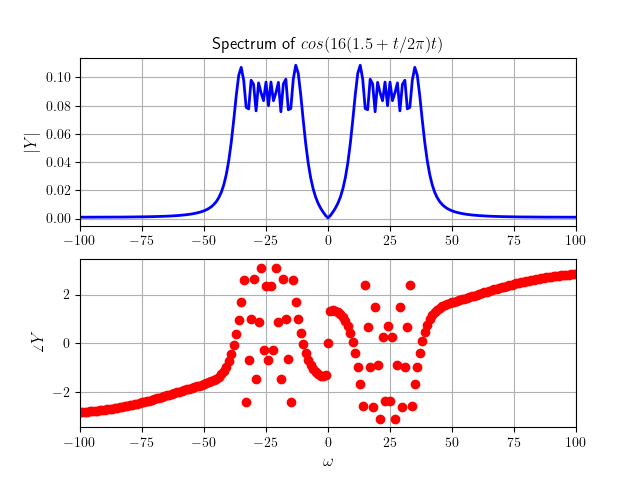
\includegraphics[width=0.8\textwidth]{q4_2.png}
\end{figure}

In the spectrum, a band is seen between 16 and 32 rads/s frequencies, but the gradual change of the frequency is not evident from the spectrum. So, a frequency - time plot is made to observe is change.

\begin{lstlisting}
def q6():
    t = np.linspace(-np.pi, np.pi, 1025); t = t[:-1]
    dt = t[1] - t[0]
    y = np.cos(16*(1.5 + t/(2*np.pi))*t)
    y[0] = 0
    # y = fftshift(y)
    piece_length = 64
    freqvstime = np.zeros((piece_length, 1024-piece_length), dtype=complex)
    for i in range(1024-piece_length):
        piece_spec = fftshift(fft(y[i:i+piece_length]))/piece_length
        freqvstime[:,i] = piece_spec
    w = np.linspace(-np.pi/dt, np.pi/dt, piece_length+1); w = w[:-1]; w = w[28:-28]
    T, W = np.meshgrid(t[piece_length//2:-piece_length//2], w)
\end{lstlisting}

The surface plot of the frequency - time plot is shown below. 

\begin{figure}[H]
\centering
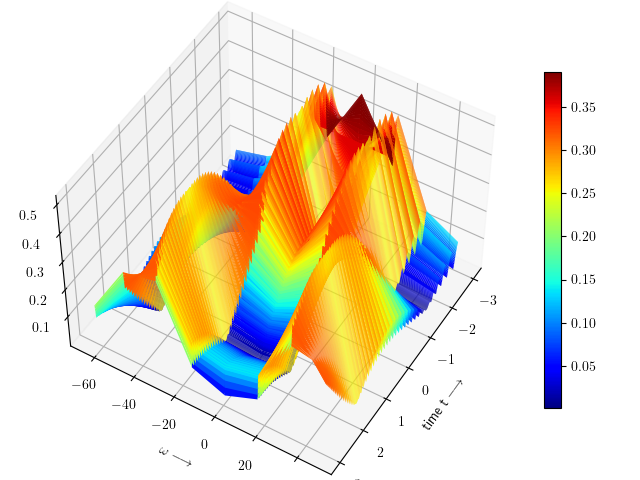
\includegraphics[width=0.8\textwidth]{q6_1.png}
\end{figure}

Instead of a surface plot, a filled contour plot gives better understanding what's happening here.

\begin{figure}[H]
\centering
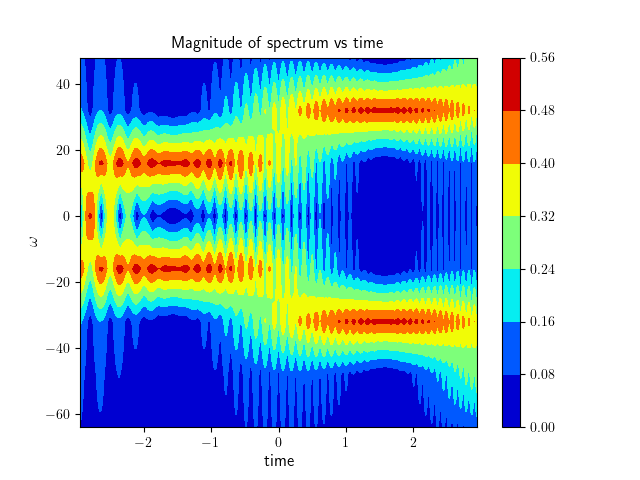
\includegraphics[width=0.8\textwidth]{q6_2.png}
\end{figure}

It can be seen that near $t = -\pi$, the peak frequency is around 16 rads/s, but this becomes 32 rads/s as $t$ becomes positive and goes towards $\pi$

\end{document} 
